%\newpage
%\thispagestyle{empty}
%~

\newpage
\thispagestyle{empty}
\vspace*{\fill}
\begin{center}
中文:11pt Adobe Song Std\\
英文:11pt Adobe Garamond Pro
\end{center}
\vspace{\fill}

\begin{titlepage}

\setlength\parindent{0pt}

\definecolor{mygreen}{HTML}{9ABA5A}
\definecolor{myblue}{HTML}{4F80BD}
\textblockcolour{mygreen}
\textblockrulecolour{white}

\begin{textblock}{6}(10,0)
    \rule{0mm}{420mm}
\end{textblock}

\begin{textblock}{.02}(9.7,0)
    \rule{0mm}{420mm}
\end{textblock}

\begin{textblock}{.02}(9.8,0)
    \rule{0mm}{420mm}
\end{textblock}

\begin{textblock}{.02}(9.9,0)
    \rule{0mm}{420mm}
\end{textblock}

\begin{textblock}{3}(11,1)
    {\Huge \textbf{雷坛巨搫}\\[5pt] \textbf{扛鼎力作}}
\end{textblock}

\begin{textblock}{12.8}(3.9,5.3)
\textblockcolour{}
    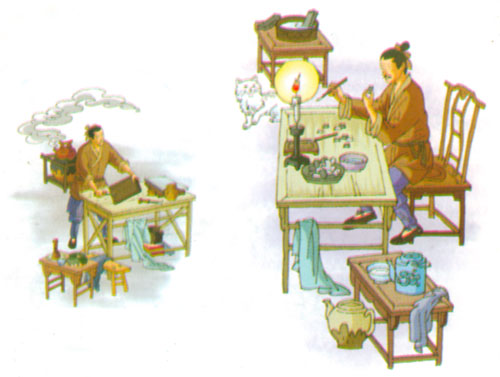
\includegraphics[scale=.9]{chinese_type.jpg}
\end{textblock}

\begin{textblock}{4}(11,13.5)
    {\huge \textit{包 太 雷}}\\[5pt]
    {\Large 2013年6月}
\end{textblock}

\TPshowboxestrue
\setlength\TPboxrulesize{0.8pt}
\textblockcolour{myblue}

\begin{textblock}{14}(0.01,3)
    \centering
    ~\\[20pt]
    {\fontsize{32}{40}\selectfont \LaTeX\ \ \textsc{Notes}}\\[8pt]
    {\huge \textit{雷太赫排版系统简介}}\\[8pt]
    第二版\ \ v2.00\\[20pt]
\end{textblock}
~
\end{titlepage}
